% \documentclass[aspectratio=169,notes]{beamer}
\documentclass[aspectratio=169]{beamer}
\usetheme[faculty=phil]{fibeamer}
\usepackage{polyglossia}
\setmainlanguage{english} %% main locale instead of `english`, you
%% can typeset the presentation in either Czech or Slovak,
%% respectively.
\setotherlanguages{russian} %% The additional keys allow
%%
%%   \begin{otherlanguage}{czech}   ... \end{otherlanguage}
%%   \begin{otherlanguage}{slovak}  ... \end{otherlanguage}
%%
%% These macros specify information about the presentation
\title[Theoretical Mechanics]{Theoretical Mechanics, Lab 13: EULER LAGRANGE} %% that will be typeset on the
\subtitle{Euler-Lagrange equation \\
\  \\ \ } %% title page.
\author{Oleg Bulichev}
%% These additional packages are used within the document:
\usepackage{ragged2e}  % `\justifying` text
\usepackage{booktabs}  % Tables
\usepackage{tabularx}
\usepackage{tikz}      % Diagrams
\usetikzlibrary{calc, shapes, backgrounds}
\usepackage{amsmath, amssymb}
\usepackage{url}       % `\url`s
\usepackage{listings}  % Code listings
% \usepackage{subfigure}
\usepackage{floatrow}
\usepackage{subcaption}
\usepackage{mathtools}
\usepackage{todonotes}
\usepackage{fontspec}
\usepackage{multicol}
\usepackage{pdfpages}
\usepackage{wrapfig}
\usepackage{animate}
\usepackage{booktabs}
\usepackage{multirow}
% \usepackage{graphicx}
\usepackage{colortbl}
\usepackage{catchfilebetweentags}
\usepackage{makecell}
\graphicspath{{resources/}}
\frenchspacing

\setbeamertemplate{caption}[numbered]
\usetikzlibrary{graphs}

% \usepackage[backend=biber,style=ieee,autocite=footnote]{biblatex}
% \addbibresource{biblio.bib}
% \DefineBibliographyStrings{english}{%
%   bibliography = {References},}

\newcommand{\oleg}[2][] {\todo[color=red, #1] {OLEG:\\ #2}}
\newcommand{\fbckg}[1]{\usebackgroundtemplate{\includegraphics[width=\paperwidth]{#1}}}%frame background

\usepackage[framemethod=TikZ]{mdframed}
\newcommand{\dbox}[1]{
\begin{mdframed}[roundcorner=3pt, backgroundcolor=yellow, linewidth=0]
\vspace{1mm}
{#1}
\vspace{1mm}
\end{mdframed}
}

\begin{document}
\setlength{\abovedisplayskip}{0pt}
\setlength{\belowdisplayskip}{0pt}
\setlength{\abovedisplayshortskip}{0pt}
\setlength{\belowdisplayshortskip}{0pt}

\fbckg{fibeamer/figs/title_page.png}
\frame[c]{\setcounter{framenumber}{0}
    \usebeamerfont{title}%
    \usebeamercolor[fg]{title}%
    \begin{minipage}[b][6.5\baselineskip][b]{\textwidth}%
        \textcolor{black}{\raggedright\inserttitle}
    \end{minipage}
    % \vskip-1.5\baselineskip

    \usebeamerfont{subtitle}%
    \usebeamercolor[fg]{framesubtitle}%
    \begin{minipage}[b][3\baselineskip][b]{\textwidth}
        \raggedright%
        \insertsubtitle%
    \end{minipage}
    \vskip.25\baselineskip
}
%   \frame[c]{\maketitle}

\fbckg{fibeamer/figs/common.png}


\section*{Theory}

\begin{frame}[t]{Generalized coordinates
    }
\framesubtitle{}
    \vspace{-0.6cm}
    \begin{figure}[H]
        \centering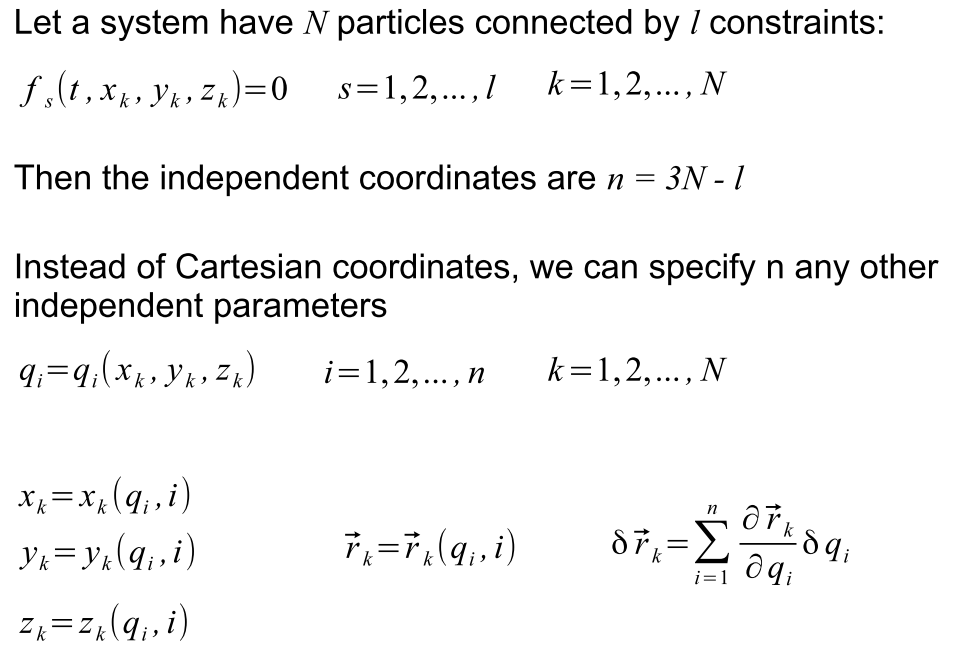
\includegraphics[height=6cm,width=1\textwidth,keepaspectratio]{image21.png}
        \label{fig:image21}
    \end{figure}
\end{frame}

\begin{frame}[t]{Generalized forces
}
\framesubtitle{}
    \vspace{-0.6cm}
    \begin{figure}[H]
        \begin{subfigure}{0.49\textwidth}
            \centering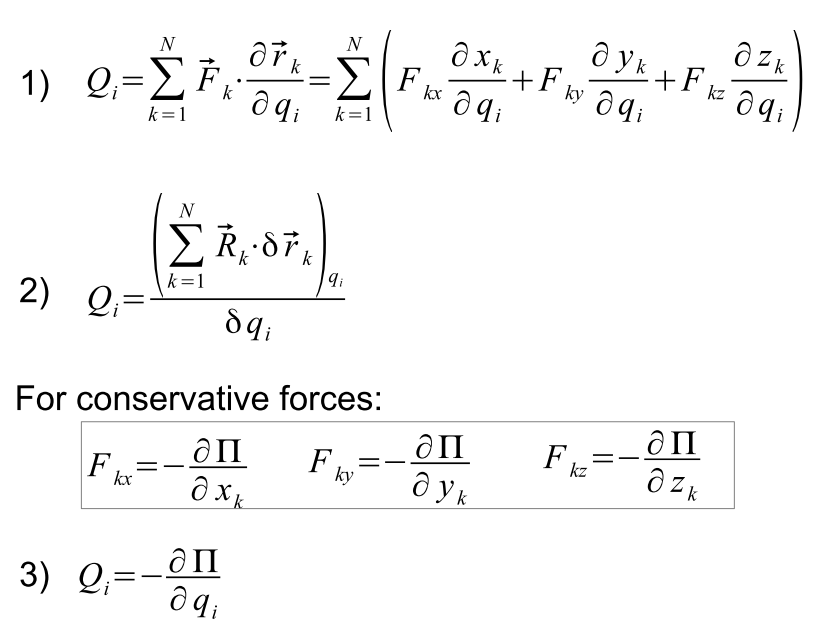
\includegraphics[height=6cm,width=1\textwidth,keepaspectratio]{image12.png}
            \label{fig:image12}
        \end{subfigure}
        \begin{subfigure}{0.49\textwidth}
            \centering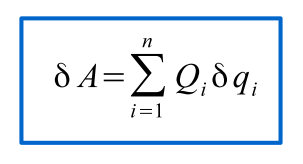
\includegraphics[height=6cm,width=0.51\textwidth,keepaspectratio]{image20.png}
            \label{fig:image20}
            \centering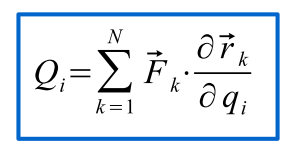
\includegraphics[height=6cm,width=0.49\textwidth,keepaspectratio]{image10.png}
            \label{fig:image10}
            \centering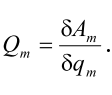
\includegraphics[height=6cm,width=0.3\textwidth,keepaspectratio]{image16.png}
            \label{fig:image16}
        \end{subfigure}
    \end{figure}
\end{frame}

\begin{frame}[t]{Euler-Lagrange equation}
    \framesubtitle{}
    \scriptsize
        \begin{tabular}{>{\centering\arraybackslash} m{0.9cm}|>{\centering\arraybackslash} m{1cm}|>{\centering\arraybackslash} m{4.0cm}|>{\centering\arraybackslash} m{2.3cm}|>{\centering\arraybackslash} m{3.8cm} } 
            \toprule
            \toprule
           \textbf{ R. O.} & \textbf{Eqn \#} & \textbf{Equations} & \textbf{Applications} & \textbf{Extra Info} \\ 
            \hline
            \ExecuteMetaData[../../dynamics_methods_overview/dynamics_methods_overview]{sndeulerlagrange}
            \bottomrule
            \bottomrule
            \end{tabular}
    \end{frame}


\section*{Tasks}

\begin{frame}[t]{Task 1 (mine)}
\framesubtitle{}
\begin{columns}[T,onlytextwidth]
    \begin{column}{0.54\textwidth}
        The system consists of body $A$, mass $m_1$ goes down without slippering. It is connected with body $C$ (mass $m_2$), using body $B$. Block $B$ rotates along the center of mass. The angle of the slope is $\alpha$.
        \medskip

        It is needed to find the acceleration of CoM $A$.
    \end{column}
    \begin{column}{0.44\textwidth}
        \begin{figure}[H]
            \centering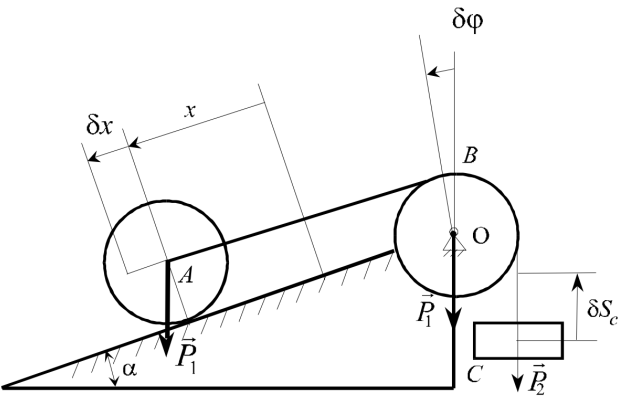
\includegraphics[height=5cm,width=1\textwidth,keepaspectratio]{image22.png}
            % \caption{caption_name}
            \label{fig:image22.png}
        \end{figure}
    \end{column}
\end{columns}
\end{frame}

\begin{frame}[t]{Task 2 (yours): Solution subfolder}
\framesubtitle{}
\small
\begin{minipage}{0.65\textwidth}
  There is a mechanical system. It moves because of gravity force. The generalized coordinates are $x$ and $\xi$. No slipping. Body $1$ is a particle. Body $3$ is a homogeneous disk;

  The goals are following:
  \begin{enumerate}
      \item find an equation of motion for this system;
      \item simulate this system (obtain all positions) or make plots for each body $x(t),\ y(t)$.
  \end{enumerate}
  Needed variables:\\
  $m_1= 1,\ m_2=3,\ m_3=2$;\\
  $b = 0.001 $, where $b$ is viscous drag coefficient;\\
  Initial conditions: $x_0=0,\ \dot{x_0}=0,\ \xi_0=0,\ \dot{\xi_0}=3$.
\end{minipage}
\begin{minipage}{0.34\textwidth}
  \begin{figure}[H]
    \centering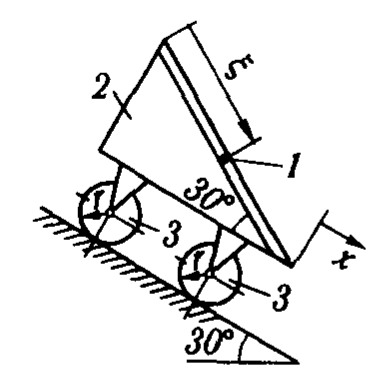
\includegraphics[height=6cm,width=1\textwidth,keepaspectratio]{HW7_1}
    \caption*{Task 2 \\ (Yablonskii (rus) D21)}
  \end{figure}
\end{minipage}
\end{frame}


\fbckg{fibeamer/figs/last_page.png}
\frame[plain]{}
\end{document}